%\documentclass[draft]{book}%%% Use for inspecting Overfull boxes.

\documentclass[twoside,a4paper]{book}

%%%%%%%%%%%%%%%%%%%%%%%%%%%%%%%%%%%%%%%%%%%%%%%%%%%%%%%%%%%
%% Currently there are very few unicode math fonts so we load fontspec %%
%% with the no-math option. This means that math fonts are defined %%%%
%% by traditional LaTeX means. Here we load the Euler fonts. %%%%%%%%%%%
%% An alternative is to delete the no-math option and enable %%%%%%%%%%
%% unicode-math and Cambria Math fonts %%%%%%%%%%%%%%%%%%%%%%%%%
%% If all else fails, you can always load the "kerkis" package %%%%%%%%%%%%
%% In any case fontspec with or without the no-math option is needed. %%
%\usepackage[no-math]{fontspec} %%%%%%%%%%%%%%%%%%%%%%%%%%%%%%%%
\usepackage{fontspec} %%%%%%%%%%%%%%%%%%%%%%%%%%%%%%%%
\usepackage{eulervm} %%%%%%%%%%%%%%%%%%%%%%%%%%%%%%%%%%%%%%%%%
%\usepackage[bold-style=tex,math-style=iso]{unicode-math} %%%%%%%%%
%\setmathfont{Cambria Math} %%%%%%%%%%%%%%%%%%%%%%%%%%%%%%%%%%%
%%%%%%%%%%%%%%%%%%%%%%%%%%%%%%%%%%%%%%%%%%%%%%%%%%%%%%%%%%%

\usepackage{xltxtra}

%%%%%%%%%%%%%%%%%%%%%%%%%%%%%%%%%%%%%%%%%%%%%%%%%%%%%%%%%
%% Language setup: The proper setup is to use the polyglossia %%%%%%%
%% package together with setting the main and other languages %%%%%%
%% and not the xgreek. However, there is still bugs and may %%%%%%%%%
%% cause problems. So we load xgreek instead but this should %%%%%%%
%% definitely change in the future. %%%%%%%%%%%%%%%%%%%%%%%%%%%%%
\usepackage{xgreek} %%%%%%%%%%%%%%%%%%%%%%%%%%%%%%%%%%%%%%%
%\usepackage{polyglossia} %%%%%%%%%%%%%%%%%%%%%%%%%%%%%%%%%%%
%\setmainlanguage{greek} %%%%%%%%%%%%%%%%%%%%%%%%%%%%%%%%%%%
%\setotherlanguage{english} %%%%%%%%%%%%%%%%%%%%%%%%%%%%%%%%%%
%%%%%%%%%%%%%%%%%%%%%%%%%%%%%%%%%%%%%%%%%%%%%%%%%%%%%%%%%

\defaultfontfeatures{Mapping=tex-text}

%%%%%%%%%%%%%%%%%%%%%%%%%%%%%%%%%%%%%%%%%%%%%%%%%%%%%%%%
%% We choose our main fonts. Fonts must be installed on the system. %
%% I.e. in /home/user/.fonts/ for Linux %%%%%%%%%%%%%%%%%%%%%%%%%
%%       in C:\Windows\Fonts\ for Winows %%%%%%%%%%%%%%%%%%%%%%%%
%% etc. We should also respect spaces in names. %%%%%%%%%%%%%%%%%%
%% So Times New Roman is not the same with TimesNewRoman %%%%%%
%\setmainfont[]{Times New Roman} %%%%%%%%%%%%%%%%%%%%%%%%%%%%%%%%%%%%
%\setmainfont[]{Cambria} %%%%%%%%%%%%%%%%%%%%%%%%%%%%%%%%%%%%
%\setsansfont[]{Candara} %%%%%%%%%%%%%%%%%%%%%%%%%%%%%%%%%%%%
%\setmonofont[]{Consolas} %%%%%%%%%%%%%%%%%%%%%%%%%%%%%%%%%%%
%\setmainfont[]{serif} %%%%%%%%%%%%%%%%%%%%%%%%%%%%%%%%%%%%

\setmainfont[]{Times New Roman} %%%%%%%%%%%%%%%%%%%%%%%%%%%%%%%%%%%%
\setsansfont[]{Times New Roman} %%%%%%%%%%%%%%%%%%%%%%%%%%%%%%%%%%%%
\setmonofont[]{Times New Roman} %%%%%%%%%%%%%%%%%%%%%%%%%%%%%%%%%%%
%%%%%%%%%%%%%%%%%%%%%%%%%%%%%%%%%%%%%%%%%%%%%%%%%%%%%%%%

%%%%%%%%%%%%%%%%%%%%%%%%%%%%%%%%%%%%%%%%%%%%%%%%%%%%%%%%%
%% If you need reverse search and your pdf viewer support this %%%%%%%
%% Currently AcrobatReader does not support this. New Linux %%%%%%%%
%% and Mac software supports this. %%%%%%%%%%%%%%%%%%%%%%%%%%%%% 
%\usepackage{pdfsync} %%%%%%%%%%%%%%%%%%%%%%%%%%%%%%%%%%%%%%
%%%%%%%%%%%%%%%%%%%%%%%%%%%%%%%%%%%%%%%%%%%%%%%%%%%%%%%%%

%%%%%%%%%%%%%%%% Use custom style %%%%%%%%%%%%%%%%
\usepackage{ptyxiakh}
%%%%%%%%%%%%%%%%%%%%%%%%%%%%%%%%%%%%%%%%%%%%%%%%%%

%%%%%%%%%%%%%%%%%%% Make index %%%%%%%%%%%%%%%%%%%
\makeindex
%%%%%%%%%%%%%%%%%%%%%%%%%%%%%%%%%%%%%%%%%%%%%%%%%%

%%%%%%%%%% Information about this work %%%%%%%%%%%
\author{Παπαδοπούλου Γεωργία}
\title{Περί ανέμων και υδάτων}
\subtitle{A Case Study}
\projectlevel{Μεταπτυχιακή Εργασία}
\date{26 Οκτωβρίου 2003}
\advisor{Όνομα καθηγητή}
\committeememberone{Καθηγητής 1}
\committeemembertwo{Καθηγητής 2}
%% leave empty if less than 3: \committeemembertwo{}
\committeememberthree{Καθηγητής 3}
\dedication{Στους γονείς μου!}
\university{Πανεπιστήμιο Αιγαίου}
\department{Τμήμα Μαθηματικών}
\def\master{ΠΡΟΓΡΑΜΜΑ ΜΕΤΑΠΤΥΧΙΑΚΩΝ ΣΠΟΥΔΩΝ}
\def\mastertitle{ΕΦΑΡΜΟΣΜΕΝΕΣ ΕΠΙΣΤΗΜΕΣ ΚΑΙ ΤΕΧΝΟΛΟΓΙΑ}
\separator{,\ }
%% another separator
%% \separator{\ $|$\ }
%% yet another one
%% \separator{\ \ding{'107}\ }
%% a simpler separator 
%% \separator{\ $\cdot$\ }
\city{Χανιά}
%%
%% University logo and scale factor. File must be in eps.
\universitylogo{%

\includegraphics[scale=1]{tuc.jpg}% University of the Aegean
%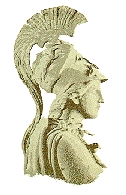
\includegraphics[scale=.6]{athina.jpg} %%%%%%% University of Athens
%\includegraphics[scale=.125]{uoc_logo.pdf} %%%%%%%% University of Crete
}
%%%%%%%%%%%%%%%%%%%%%%%%%%%%%%%%%%%%%%%%%%%%%%%%%%

%%%%%%%%%%%% New theorems %%%%%%%%%%%%%%%%%%%%%%%%
\newtheorem{theorem}{Θεώρημα}[section]         
\newtheorem{lemma}[theorem]{Λήμμα}
\newtheorem{proposition}[theorem]{Πρόταση}
\newtheorem{corollary}[theorem]{Πόρισμα}
\newtheorem{definition}[theorem]{Ορισμός}
\newtheorem{remark}[theorem]{Παρατήρηση}
%%%%%%%%%%%%%%%%%%%%%%%%%%%%%%%%%%%%%%%%%%%%%%%%%%%
%Αυτα τα προσθεσα εγώ!
%\usepackage{amsmath}
%\usepackage{amssymb}
%\usepackage{yhmath}
%\usepackage{amsthm}
\usepackage{graphicx}

\usepackage{pdfpages}

%%%%%%%%%%%%%%%%%%%%% Document starts %%%%%%%%%%%%
\begin{document}
%%%%%%%%%%%%%%%%%%%%%%%%%%%%%%%%%%%%%%%%%%%%%%%%%%

%%%%%%%%%%%%%%%%%%%%%%% Start Roman numbering %%%%
%%%%%%%%%%%%%%%%%%%%%%%%%%%%%%%%%%%%%%%%%%%%%%%%%%

\includepdf[pages={1}]{eksofyllo.pdf}

\pagenumbering{roman}
%\makecover  % Eksofyllo
%%%%%%%%%%%%%%%%%%% Table of contents %%%%%%%%%%%%
\tableofcontents
%%%%%%%%%%%%%%%%%%%%%%%%%%%%%%%%%%%%%%%%%%%%%%%%%%

%%%%%%%%%%%%%%%%%%%%%%%%%%%%%%%%%%%%%%%%%%%%%%%%%%%%%%%%%%%%%
\chapter*{ΕΙΣΑΓΩΓΗ}
\addcontentsline{toc}{chapter}{ΕΙΣΑΓΩΓΗ}
%%%%%%%%%%%%%%%%%%%%%%%%%%%%%%%%%%%%%%%%%%%%%%%%%%%%%%%%%%%%%

Εδώ η Γεωργία θα γράψει την εισαγωγή της. Στην πορεία θα συζητήσουμε
την δομή της εισαγωγής~\cite{Kourounis2014}. 
Πρέπει η εισαγωγή να έχει παρόμοιο θεματικό σκελετό με την~\cite{Jansen:book,Chen:2012} 
περίληψη και τα συμπεράσματα στο τέλος της εργασίας.\\ \\
Το αντικείμενο είναι λοιπόν η ανάλυση χρονοσειρών,
δηλαδή η χρήση μεθόδων που θα μας επιτρέψουν να διερευνήσουμε το μηχανισμό
(στοχαστική διαδικασία ή δυναμικό σύστημα) που παράγει τη χρονοσειρά, να
εκτιμήσουμε χαρακτηριστικά του, να αναπτύξουμε μοντέλο για να το περιγράψουμε
και να κάνουμε προβλέψεις της εξέλιξης του, δηλαδή τις επόμενες τιμές στη
χρονοσειρά.




\bigskip

\begin{flushright}
\begin{minipage}{150pt}
Γ.\ Παπαδοπούλου, Χανιά 2015.
\end{minipage}
\end{flushright}



\endinput
%%% Local Variables: 
%%% mode: latex
%%% TeX-master: "ptyxiakn"
%%% End: 


\cleardoublepage

%%%%%%%%%%% Return to normal numbering %%%%%%%%%%%
\pagenumbering{arabic}
%%%%%%%%%%%%%%%%%%%%%%%%%%%%%%%%%%%%%%%%%%%%%%%%%%

%%%%%%%%%%%%%%%%%%%%%%%%%% Part One %%%%%%%%%%%%%%%%
\part{ΑΝΑΛΥΣΗ ΧΡΟΝΟΣΕΙΡΩΝ}
%%%%%%%%%%%%%%%%%%%%%%%%%%%%%%%%%%%%%%%%%%%%%%%%%%%%


%%%%%%%%%%%%%%%%%%%%%%%%%%%%%%%%%%%%%%%%%%%%%%%%%%%%%%%%%%%%%%%%%%%%%%%%%%%%
\chapter{ΒΑΣΙΚΕΣ ΕΝΝΟΙΕΣ ΧΡΟΝΟΣΕΙΡΑΣ}
%%%%%%%%%%%%%%%%%%%%%%%%%%%%%%%%%%%%%%%%%%%%%%%%%%%%%%%%%%%%%%%%%%%%%%%%%%%%



%%%%%%%%%%%%%%%%%%%%%%%%%%%%%%%%%%%%%%%%%%%%%
\section{Η ΕΝΝΟΙΑ ΤΗΣ ΧΡΟΝΟΣΕΙΡΑΣ}
%%%%%%%%%%%%%%%%%%%%%%%%%%%%%%%%%%%%%%%%%%%%%
 Η χρονοσειρά μπορεί να ορισθεί ως μια συλλογή διαδοχικών χρονικών
παρατηρήσεων της τιμής κάποιου μεγέθους. Πρόκειται ουσιαστικά για μια στοχαστική
διαδικασία, μιας και η εξέλιξη των τιμών του μεγέθους επηρεάζεται από τυχαίους
παράγοντες, ενώ η τιμή κάθε χρονικής στιγμής συνιστά και μια ξεχωριστή τυχαία
μεταβλητή. Με τον όρο χρονοσειρά δηλαδή, εννοούμε συνήθως μια ακολουθία $\{ x_t : t = 0,1,2,\ldots \}$ , όπου
κάθε $ x_t $ εκφράζει την κατά την χρονική στιγμή $ t $ κατάσταση ενός συστήματος το
οποίο εξελίσσεται στο χρόνο κατά τυχαίο εν γένει τρόπο (stochastic system).\\ 
Παραδείγματα τέτοιων χρονοσειρών είναι: \\
\begin{enumerate}


\item Οι ημερήσιες, αεροπορικές και οδικές, αφίξεις τουριστών στην χώρα μας $ x_t $ με
$t = 1, 2,\ldots $
\item Ο αριθμός $ x_t $ πελατών μέσα σε ένα πολυκατάστημα κατά τη χρονική στιγμή
$ t $ με $ t \in [0, T ] $.
\item Ο συνολικός αριθμός τροχαίων ατυχημάτων $ x_t $ κατά μήκος μιας οδικής
αρτηρίας στο χρονικό διάστημα [0,t] με t ≥ 0.
\item Η ημερήσια κατανάλωση ηλεκτρικού ρεύματος καθώς και η ημερήσια
κατανάλωση ύδατος, $ x_t $ και $ y_t $ αντίστοιχα, σε μια μεγάλη γεωγραφική περιοχή
της χώρας με $ t = 1, 2,\ldots $

\item Οι οικονομικές χρονοσειρές, όπως το ετήσιο ακαθάριστο εθνικό προϊόν και
ετήσιο ισοζύγιο εξωτερικών συναλλαγών $ x_t $ και $ y_t $ αντίστοιχα, με $ t = 1, 2,\ldots $
\item Οι μετεωρολογικές χρονοσειρές, όπως η θερμοκρασία περιβάλλοντος και
ατμοσφαιρική πίεση, $ x_t $ και $ y_t $ αντίστοιχα, σε συγκεκριμένη γεωγραφική
περιοχή με γεωγραφικές συντεταγμένες $ \left(l, a, h \right) $ κατά την χρονική στιγμή $ t $.
Εδώ η χρησιμοποιούμενη παράμετρος $ t $ είναι περισσότερο σύνθετη και
συγκεκριμένα $ t = \left( l,a,h ,t \right) $.
\end{enumerate}
%%%%%%%%%%%%%%%%%%%%%%%%%
%%%%%%%%%%%%%%%%%%%%%%%
%%%%%%%tha taa ksanadwwwwwwwwwww

Όπως διαπιστώνει κανείς από τα παραπάνω παραδείγματα, οι χρονοσειρές μπορούν
να αφορούν διακριτά μεγέθη $ x_t $ σε διακριτό χρόνο t, περίπτωση (i), διακριτά μεγέθη
$ x_t $ σε συνεχή χρόνο t, περιπτώσεις (ii) και (iii), συνεχή μεγέθη $x_t$ σε διακριτό χρόνο t, περιπτώσεις (iv) και (v) και συνεχή μεγέθη $x_t$ σε συνεχή χρόνο t, περίπτωση (vi).
Το πρόβλημα είναι η “πρόβλεψη” μελλοντικών τιμών της χρονοσειράς με βάση τις
μέχρι σήμερα τιμές τις ίδιας χρονοσειράς, περιπτώσεις (i)-(iii), είτε ακόμα και σε
συνδυασμό με τις μέχρι σήμερα τιμές μιας άλλης χρονοσειράς η οποία εξελίσσεται
παράλληλα με την πρώτη και επιδρά πάνω σ ́ αυτή, περιπτώσεις (iv)-(vi), οπότε
μιλάμε για πολυμεταβλητές χρονοσειρές. Το σύνολο των δυνατών καταστάσεων
ονομάζεται χώρος καταστάσεων και συμβολίζεται με S, ένα (μονοδιάστατο)
υποσύνολο του  $ R $   , ή γενικότερα ένα πολυδιάστατο υποσύνολο του $ R^d $, ενώ το
σύνολο τιμών του t ονομάζεται παραμετρικός χώρος, συμβολίζεται με Τ και μπορεί
επίσης να είναι υποσύνολο του $ R^k $, όταν χρειάζεται ένα πολυδιάστατο t για να
καθορίσουμε πέραν του χρόνου t και γεωγραφικές π.χ. συντεταγμένες $\left( l,a,h \right)$ σε
χωρο-χρονοσειρές (spatial time series), βλ. παράδειγμα (vi) παραπάνω. Σημειώνεται
οι όροι διακριτά και συνεχή μεγέθη είναι σε αντιστοιχία με τους όρους διακριτές και
συνεχείς τυχαίες μεταβλητές. \\ \\
Ένα παράδειγμα μίας χρονοσειράς απεικονίζεται στο ακόλουθο σχήμα 1.1, όπου παρουσιάζεται το γράφημα
της ετήσιας τιμής του αργού πετρελαίου σε αμερικανικά δολάρια ανά βαρέλι. Ο χρονικός ορίζοντας είναι 117 χρόνια, από το έτος 1870 έως το έτος 1987. Το γράφημα ελήφθη από το βιβλίο των R. Pindyck και
D. Rubinfeld (1998).\\\\
\begin{center}
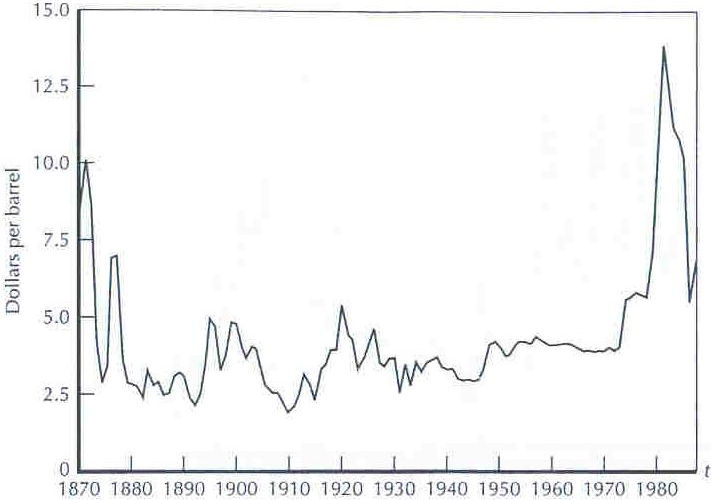
\includegraphics[scale=0.4]{graf1.png}\\   
\textbf{Σχήμα 1.1: Γράφημα χρονοσειράς τιμής αργού πετρελαίου σε δολάρια ανά βαρέλι.}
\end{center} 
\linespread{1}



Η συστηματική μελέτη μιας χρονοσειράς ξεκινάει με την επισκόπηση του
γραφήματός της στο πεδίο του χρόνου, από το οποίο μπορούν αρχικά να ανιχνευθούν
τρία βασικά ποιοτικά χαρακτηριστικά της: Η τάση, η εποχικότητα και οι ακραίες
παρατηρήσεις.\\
\begin{itemize}

\item Η \textbf{τάση} (trend) γενικά θα μπορούσε να ορισθεί ως η μακροπρόθεσμη μεταβολή του
μέσου επιπέδου των τιμών μιας χρονοσειράς. Έτσι, μπορεί η τάση των τιμών να είναι
αυξητική, πτωτική ή σταθερή σε ένα συγκεκριμένο χρονικό διάστημα, ενώ μπορεί και να
έχει τη μορφή κάποιας συνάρτησης στο εν λόγω διάστημα. Να σημειωθεί ότι η έννοια
“μακροπρόθεσμη μεταβολή” εξαρτάται από την εκάστοτε εφαρμογή που εξετάζεται.
\item Η \textbf{εποχικότητα} (seasonal) μπορεί να ορισθεί σαν μια περιοδική διακύμανση που έχει
σταθερό μήκος. Η εν λόγω διακύμανση τις περισσότερες φορές διακρίνεται εύκολα και
μπορεί να ερμηνευθεί στα πλαίσια του υπό μελέτη φαινομένου. Φερ' ειπείν, αν
κανείς επιθυμούσε να αναλύσει τη χρονοσειρά των τιμών των καυσίμων σε βάθος
χρόνων, είναι λογικό να περιμένει να παρατηρήσει μια σχετική άνοδο κατά τους
χειμερινούς μήνες κάθε έτους.

\item Οι \textbf{ακραίες παρατηρήσεις} (outliers) είναι οι απομονωμένες παρατηρήσεις που
εμφανίζονται στο γράφημα κάποιας χρονοσειράς ως απότομες αλλαγές στο πρότυπο
συμπεριφοράς της. Τα outliers μελετήθηκαν αρχικά κατά κύριο λόγο από τον A. J. Fox
(1972), ο οποίος μάλιστα εισήγαγε δύο τύπους. Ο τύπος I αφορά περιπτώσεις όπου η
ύπαρξη μιας ακραίας τιμής δεν έχει καμία επίδραση στις ακόλουθες παρατηρήσεις.
Αντιθέτως, ο τύπος ΙΙ αφορά περιπτώσεις όπου υπάρχει επίδραση στη μετέπειτα
συμπεριφορά των τιμών της χρονοσειράς, παράγοντας μια σειρά λιγότερο ή περισσότερο
ακραίων παρατηρήσεων ή αλλάζοντας εξ’ ολοκλήρου τα χαρακτηριστικά της.
\end{itemize}

Για την ανάλυση της χρονοσειράς εντοπίζουμε τα μοτίβα των διαθέσιμων δεδομένων
(δηλ, της χρονοσειράς) προκειμένου να καταλάβουμε τον τρόπο με τον οποίο
συμπεριφέρονται. Ακριβώς σε αυτή τη συμπεριφορά βασίζεται η πρόβλεψη. Αυτά τα
μοτίβα μπορεί να είναι:\\
\begin{enumerate}
\item επίπεδο (level): ένα τέτοιο μοτίβο υπάρχει όταν τα δεδομένα κυμαίνονται
γύρω από μία μέση τιμή.\\
\begin{center}
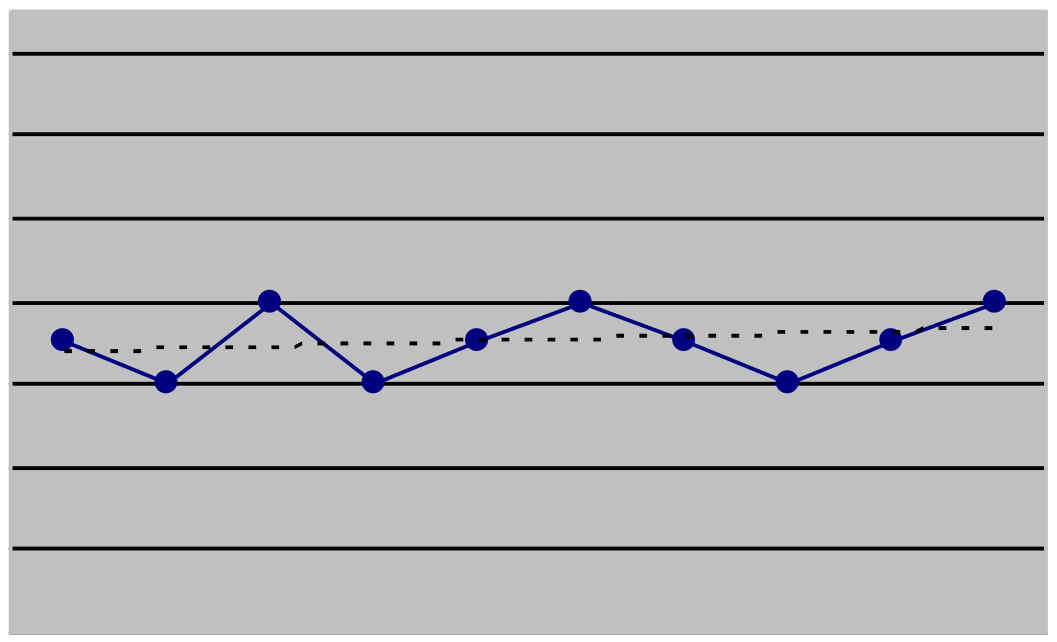
\includegraphics[scale=0.2]{level.png}\\
\end{center}
\item τάση (trend): είναι η σταδιακή ανοδική ή πτωτική κίνηση των δεδομένων στο
χρόνο. Η κίνηση αυτή μπορεί να είναι γραμμική, εκθετική κτλ.\\
\begin{center}
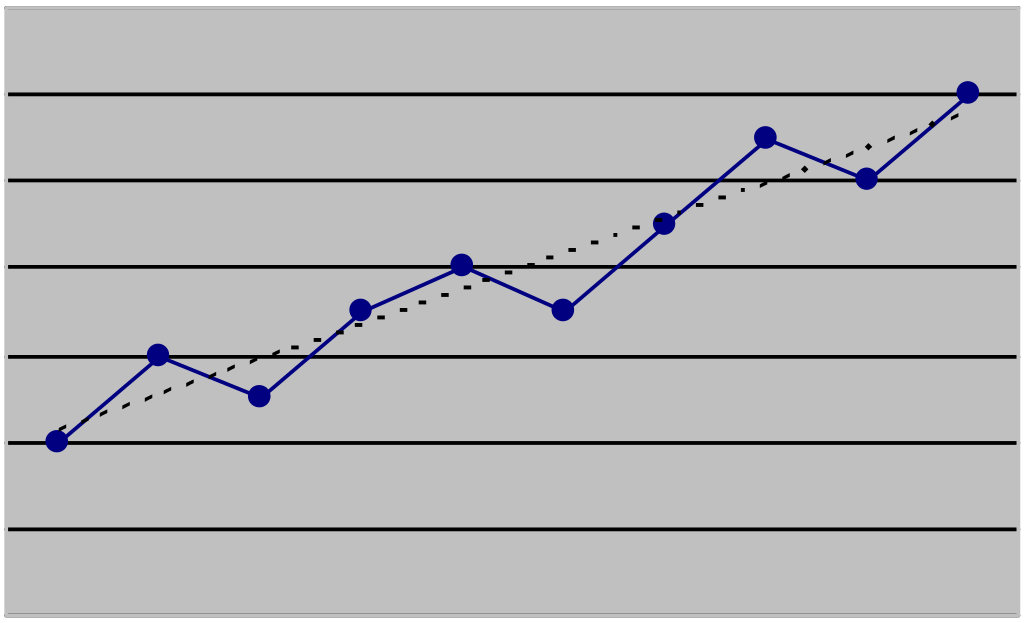
\includegraphics[scale=0.2]{trend.png}
\end{center}
\item εποχικότητα (seasonality): είναι η κανονικά επαναλαμβανόμενη κίνηση των
δεδομένων μέσα σε σχετικά μικρό χρονικό διάστημα (συνήθως μέσα σε ένα
χρόνο). Τέτοιο μοτίβο μπορεί να παρουσιάζουν οι μεταβλητές που
επηρεάζονται από εποχικούς παράγοντες: π.χ. οι πωλήσεις παγωτών αυξάνουν
κατά τους ζεστούς μήνες και μειώνονται κατά τους κρύους.
\begin{center}
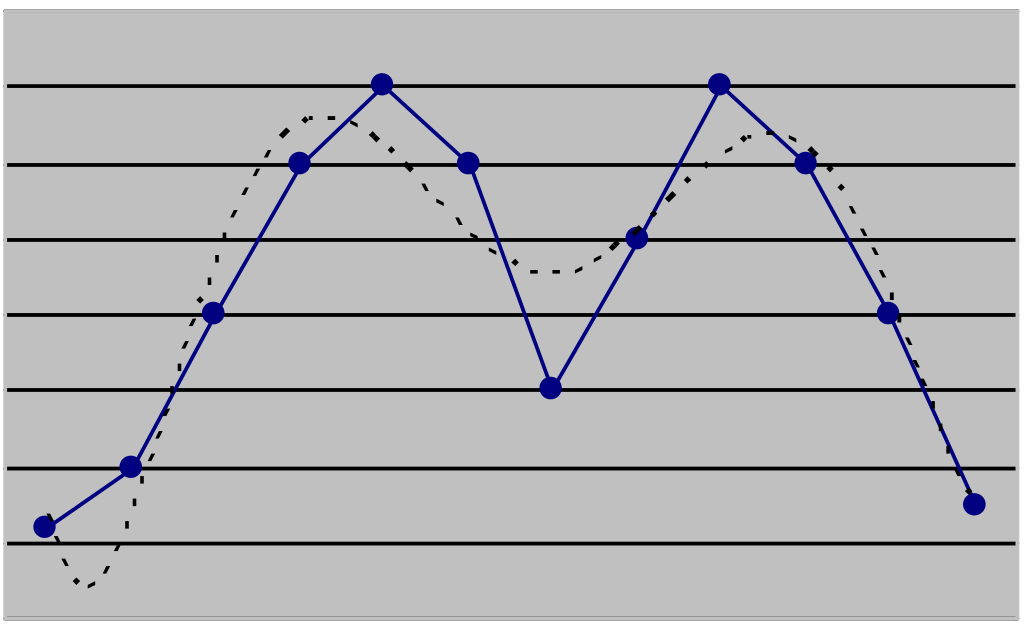
\includegraphics[scale=0.2]{season.png}
\end{center}
\item κυκλικότητα (cycle): είναι (όπως και η εποχικότητα) η επαναλαμβανόμενη
αυξομείωση των δεδομένων, με μεγαλύτερο όμως χρονικό ορίζοντα (5-10
χρόνια), και είναι συνήθως συνδεδεμένη με τις διακυμάνσεις στο επίπεδο της
συνολικής οικονομίας (γνωστές ως περίοδοι οικονομικής ύφεσης και
οικονομικής ανάπτυξης).\\
\begin{center}
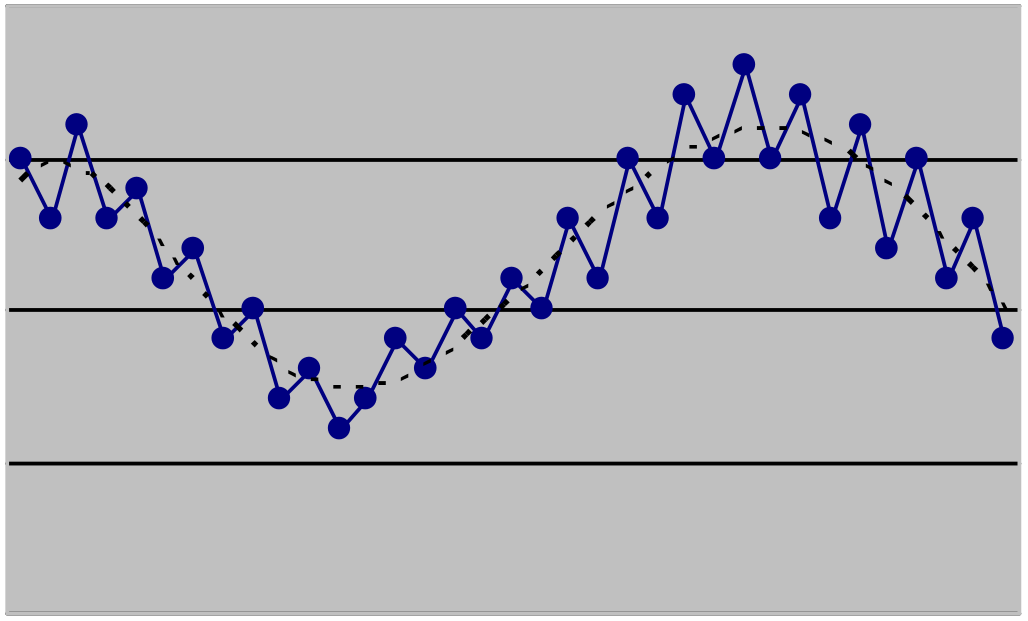
\includegraphics[scale=0.2]{cycle.png}
\end{center} 
\item τυχαιότητα (randomness): είναι η κίνηση των δεδομένων που δεν παρουσιάζει
καμία κανονικότητα.
\end{enumerate}
Αν εξετάσουμε μια οποιαδήποτε χρονοσειρά, διαπιστώνουμε ότι αποτελεί συνδυασμό
ενός ή περισσότερων από τα παραπάνω στοιχεία.\\
Στο παρακάτω διάγραμμα φαίνεται μια χρονοσειρά με εμφανή την ύπαρξη αυξητικής
τάσης και, ταυτόχρονα, εποχικότητας.\\
\begin{center}
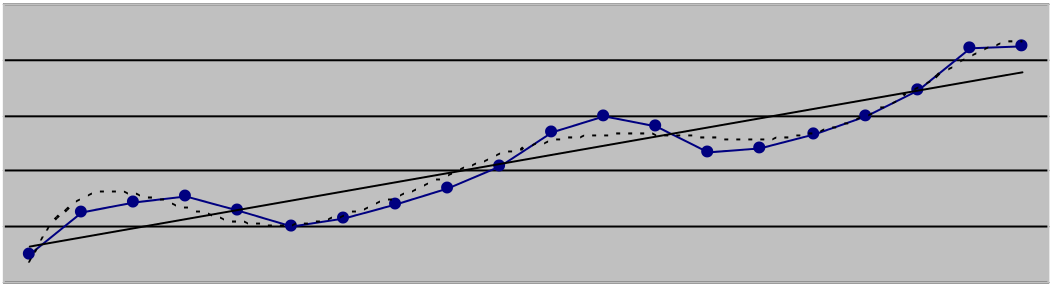
\includegraphics[scale=0.3]{graf4.png}
\end{center}



%%%%%%%%%%%%%%%%%%%%%%%%%%%%%%%%%%%%%%%%%%%%%%%
\section{ΣΤΟΧΑΣΤΙΚΕΣ ΑΝΕΛΙΞΕΙΣ}
%%%%%%%%%%%%%%%%%%%%%%%%%%%%%%%%%%%%%%%%%%%%%%%
Όπως ήδη αναφέραμε, χρονοσειρά είναι μια ακολουθία τιμών
$\{ x_t : t = 0,1,2,\ldots\}$ η οποία εκφράζει την εξέλιξη ενός στοχαστικού συστήματος, ενός
συστήματος δηλαδή με τυχαία κατά μάλλον ή ήττον συμπεριφορά, σε αντίθεση με
αυτήν ενός προσδιοριστικού (deterministic) συστήματος, η οποία συνήθως
περιγράφεται από ένα σύστημα διαφορικών εξισώσεων. Όπως είναι γνωστό από την
Θεωρία των Στοχαστικών Ανελίξεων, η εξέλιξη ενός στοχαστικού συστήματος
μπορεί να περιγραφεί πιθανοθεωρητικά μέσω μιας στοχαστικής ανέλιξης (σ.α.),
μονοδιάστατης ή πολυδιάστατης, δηλαδή μιας ακολουθίας τυχαίων μεταβλητών
$\{X_n : n \in N \}$ , ή γενικότερα μιας (υπεραριθμήσιμης) οικογένειας τυχαίων
μεταβλητών $\{X_t : t \in T \}$ , που ορίζεται πάνω σε ένα χώρο πιθανότητας $\left(\Omega , F , P \right)$ .

Σημειώνεται ότι για δεδομένο $\omega \in \Omega$ , η $ \{x_t=X_t\left(\omega\right):t \in T\}$ εκφράζει μια
συνάρτηση του χρόνου t και αποτελεί την τροχιά ή πραγματοποίηση (sample path,
realization) της σ.α. $\{ X_t : t \in T \}$ . Συνεπώς, ο όρος χρονοσειρά
χρησιμοποιείται τόσο για μια στοχαστική ανέλιξη $\{ X_t : t \in T \}$, όσο και για μία
τροχιά $ \{x_t=X_t\left(\omega\right):t \in T\}$.

%%%%%%%%%%%%%%%%%%%%%%%%%%%%%%%%%%%%%%%%%%%%%%%%%%%%%%
\section{ΚΑΤΑΝΟΜΕΣ ΚΑΙ ΡΟΠΕΣ ΣΤΟΧΑΣΤΙΚΗΣ ΔΙΑΔΙΚΑΣΙΑΣ }
%%%%%%%%%%%%%%%%%%%%%%%%%%%%%%%%%%%%%%%%%%%%%%%%%%%%%%
Η ακολουθία των τυχαίων μεταβλητών $Y_t$ για κάθε χρονική στιγμή t ορίζει τη
στοχαστική διαδικασία $ \{Y_t\}_{t=-\infty}^{+\infty}$(και αντίστοιχα για τη $X_t$ και $ \{X_t\}_{t=-\infty}^{+\infty}$ ). Θα
αναφερόμαστε στη στοχαστική διαδικασία και ως χρονοσειρά εννοώντας την
άγνωστη ακολουθία των τυχαίων μεταβλητών και όχι τις παρατηρήσεις. \\ \\
Η πλήρης περιγραφή μιας στοχαστικής διαδικασίας $\{Y_t\}_{t=-\infty}^{+\infty} $ απαιτεί ότι οι κοινές
κατανομές όλων των τάξεων
 είναι γνωστές για κάθε χρονική στιγμή t.
Η κατανομή τάξης ένα αντιστοιχεί στη στατική περιγραφή της στοχαστικής
διαδικασίας και είναι η (περιθώρια) κατανομή της $\{Y_t\}_{t=-\infty}^{+\infty} $\\
$$ \forall t \in Z, \quad f_{Y_t}\left(y\right)=f_Y\left(y,t\right),$$
δηλαδή ορίζεται ως συνάρτηση όχι μόνο της κάθε τιμής $y$ αλλά και του χρόνου t. Κατά τον ίδιο τρόπο η κοινή κατανομή δύο μεταβλητών της $\{Y_t\}_{t=-\infty}^{+\infty} $ (κατανομή τάξης
2) είναι\\
$$ \forall t_1,t_2 \in Z,\quad f_{Y_{t1},Y_{t2}} \left(y_1,y_2\right)= f_Y\left(y_1,y_2,t_1,t_2\right)$$.






Δεδομένου ότι μια χρονοσειρά αποτελεί μια στοχαστική διαδικασία,
δηλαδή κάθε παρατήρησή της αποτελεί μια τυχαία μεταβλητή,
υποθέτουμε ότι μελετούμε την χρονική εξέλιξη των τιμών ενός μεγέθους $Υ$. Έτσι,
την χρονική στιγμή t η τιμή του μεγέθους θα είναι μια τυχαία μεταβλητή $Y_t$ με
συνάρτηση πυκνότητας πιθανότητας
$f_{Y_t} \left(y_t \right)$. Έστω ακόμη ότι έχουμε παρατηρήσει ένα
δείγμα τιμών μεγέθους Τ, δηλαδή έχουμε συλλέξει τις τιμές για $t = 1, 2,\ldots,T$
$$\{ Y_1,Y_2,\ldots,Y_T \} $$

Το παραπάνω δείγμα τιμών αναπαριστά μια συγκεκριμένη “έκβαση” της στοχαστικής
διαδικασίας που γεννά τα δεδομένα. Αν τώρα η εν λόγω στοχαστική διαδικασία Υ
επαναληφθεί Ν ανεξάρτητες φορές, θα έχουμε ένα σύνολο Ν “πραγματοποιήσεων” όλων
των παρατηρήσεων – τυχαίων μεταβλητών $Υ_t$ που συνθέτουν τη χρονοσειρά. Συνεπώς,
όσον αφορά το παραπάνω δείγμα τιμών μεγέθους Τ, για την κάθε μία παρατήρηση $Y_t$ θα
έχουμε το εξής σύνολο\\
$$ \{Y_t^{\left(1\right)},Y_t^{\left(2\right)},\ldots, Y_t^{\left(N\right)}\},\quad \forall t=1,2,\ldots,T$$


Η μέση τιμή (ροπή πρώτης τάξης) ή  αναμενόμενη τιμή $\mu_t$ της t–οστής παρατήρησης (τυχαίας μεταβλητής) $Y_t$
της παραπάνω χρονοσειράς Υ δίδεται από τη σχέση:\\
$$\mu = E \left[  Y_t \right]= \int_{-\infty }^{+\infty } y_tf_{Y_t}\left(y_t\right) dy   $$



Η μέση τιμή $\mu_t$ σχετίζεται άμεσα
με την έννοια της \textit{τάσης} της χρονοσειράς, εφόσον εκφράζεται ως συνάρτηση της
χρονικής στιγμής $t$ της παρατήρησης $Y_t$ . Συγκεκριμένα, αν μια χρονοσειρά παρουσιάζει
αυξητική ή πτωτική τάση αντιστοίχως σε ένα χρονικό διάστημα, αυτό θα αποτυπώνεται
και στη μέση τιμή της $\mu_t$ ως συνάρτηση του χρόνου. Ακόμη, η μη ύπαρξη τάσης σε ένα
χρονικό διάστημα αποτυπώνεται στη σταθερή αναμενόμενη τιμή $\mu_t$ στο εν λόγω
διάστημα.
%
%\textbf{Η διασπορά}:\\ $$\sigma^2\left( t \right) =V \left[X_t \right] = E\left[\left( X_t-\mu_t\right) ^2  \right], \quad t \in T    $$
%
% \textbf{Η αυτοσυνδιακύμανση}:\\
%$$ \gamma\left(t,h \right) = Cov\left(X_t,X_{t+h} \right) =E\left[ \left(X_t-\mu_t \right)\left( X_{t+h}-\mu_{t+h}\right)  \right], \quad t,h \in T   $$ 
%
%Είναι προφανές ότι ισχύει: 
%$\sigma^2\left( t \right)=\gamma\left( t,0\right) =Cov\left(X_t,X_t \right),\quad t,h \in T   $ \\
%Είναι γνωστό επίσης ότι όταν οι διασπορές δύο τυχαίων μεταβλητών Χ και Υ , είναι
%πεπερασμένες, τότε τόσο οι μέσες τιμές αυτών όσο και η συνδιακύμανση αυτών
%είναι πεπερασμένες ποσότητες. Τούτο διότι αφενός πρέπει να έχουμε\\
%$E \left[ \vert X \vert ^2 \right]< ∞ , E \left[ \vert X \vert ^2 \right] < ∞ $, αφού διαφορετικά δεν ορίζονται οι διασπορές, και αφετέρου,
%με εφαρμογή της ανισότητας Cauchy-Schwarz\\
%$$E \left[\vert X \vert\vert Y \vert \right] \leq \sqrt{ E \left[ X^2 \right] E \left[ Y^2 \right]}, $$
%προκύπτει:\\
%$$\vert E \left[ X \right] \vert \leq E \left[\vert X \vert \right] \leq \sqrt{ E \left[ X^ 2 \right]} < ∞ , \quad \vert E \left[ Y \right] \vert \leq E \left[\vert Y \vert\right] \leq \sqrt{ E \left[ Y^ 2 \right]} < ∞  ,$$
%και
%$$ \vert Cov \left( X , Y \right) \vert \leq \sqrt{ V \left[ X \right] V \left[ Y \right]} < ∞ .$$


%\subsection{ΑΥΤΟΣΥΝΔΙΑΚΥΜΑΝΣΗ}
%\subsection{ ΑΥΤΟΣΥΣΧΕΤΗΣΗ}

%%%%%%%%%%%%%%%%%%%%%%%%%%%%%%%%%%%%%%%%%%%%%
\section{ ΣΤΑΣΙΜΟΤΗΤΑ ΚΑΙ ΑΥΤΟΣΥΣΧΕΤΗΣΗ}
%%%%%%%%%%%%%%%%%%%%%%%%%%%%%%%%%%%%%%%%%%%%%
Η στατιστική περιγραφή της στοχαστικής διαδικασίας απλουστεύεται αν
θεωρήσουμε ότι οι στατιστικές της ιδιότητες παραμένουν σταθερές στο χρόνο και
τότε η στοχαστική διαδικασία ορίζεται ως στάσιμη. Αυτή είναι μα υπόθεση που
δύσκολα μπορεί να υιοθετηθεί σε πολλά πραγματικά προβλήματα, αλλά μπορεί να
χρησιμοποιηθεί ως υπόθεση εργασίας για την εξαγωγή χρήσιμων συμπερασμάτων.\\ \\
Ειδικότερα ορίζονται δύο μορφές στασιμότητας:\\


%Η ύπαρξη μη-στασιμότητας είναι ένα από τα βασικότερα προβλήματα στην
%ανάλυση χρονοσειρών.

%Είναι φανερό ότι έχοντας παρατηρήσει μια χρονοσειρά
%$ \{ X_t : t \in T \} $
%από κάποια
%χρονική στιγμή $ t = 0 $, έστω μέχρι και την παρούσα χρονική στιγμή $ t = s $, αν δηλαδή
%γνωρίζουμε την τροχιά αυτής $ \{ X_t : 0 \leq t \leq s \}$ , και θέλουμε να προβλέψουμε
%μελλοντικές τιμές αυτής $ X_{s + h} $, με $ h > 0 $, θα πρέπει να βασιστούμε στις μέχρι τώρα
%γνωστές τιμές της και στην εξάρτηση που ενδέχεται να υπάρχει μεταξύ $ X_{s + h} $ και
%των τιμών
%$ \{ X_t : 0 \leq t \leq s \}$
%της χρονοσειράς στο παρελθόν. Τούτο βέβαια με την
%προϋπόθεση ότι όλα τα πιθανοθεωρητικά χαρακτηριστικά μιας χρονοσειράς, ή
%τουλάχιστον τα βασικότερα εξ αυτών, παραμένουν αναλλοίωτα στον χρόνο. \\ \\
%Όταν όλα τα πιθανοθεωρητικά χαρακτηριστικά μιας χρονοσειράς παραμένουν
%αναλλοίωτα στο χρόνο τότε μιλάμε για \textit{αυστηρή στασιμότητα}. Συγκεκριμένα έχουμε:
%\begin{enumerate}
\begin{dinglist}{43}
\item \textbf{ Αυστηρή Στασιμότητα} \\\\
Η στοχαστική διαδικασία $\{Y_t\}_{t=-\infty}^{+\infty}$
 είναι αυστηρά στάσιμη όταν οι κατανομές της για
κάθε τάξη (ή ισοδύναμα όλες οι ροπές) είναι σταθερές στo χρόνο, δηλαδή όταν ισχύει:\\ \\
$ \forall t \in Z, \quad f_{Y_t}\left(y\right)=f_Y\left(y,t\right)=f_Y\left(y\right) $\\
$ \forall t_1,t_2 \in Z, \quad f_{Y_{t1},Y_{t2}} \left(y_1,y_2\right)=f_{Y_t,Y_{t-\tau}}\left(y_1,y_2\right) $\\
$\forall t_1,t_2,t_3 \in Z, \quad f_{Y_{t1},Y_{t2},Y_{t3}} \left(y_1,y_2,y_3\right)=f_{Y_t,Y_{t-\tau1},Y_{t-\tau2}}\left(y_1,y_2,y_3\right)$\\\\
και αντίστοιχα για κατανομές μεγαλύτερης τάξης.\\

Για ροπές τάξης μεγαλύτερης του ένα, οι κατανομές δίνονται ως συνάρτηση όχι των
χρονικών στιγμών, π.χ. $t_1 , t_2$ , αλλά της υστέρησης μεταξύ των χρονικών στιγμών, π.χ. $\tau=t_2-t_1$ , δηλαδή για οποιεσδήποτε δύο χρονικές στιγμές που απέχουν μεταξύ τους $\tau$
χρονικά βήματα. Ο έλεγχος της αυστηρής στασιμότητας απαιτεί τη διερεύνηση
κοινών κατανομών ή ροπών όλων των τάξεων και δεν αποτελεί μια πρακτικά χρήσιμη
ιδιότητα. Για αυτό συχνά χαλαρώνουμε τη συνθήκη στασιμότητας περιορίζοντας την
στις δύο πρώτες ροπές.\\

%Η χρονοσειρά $\: \{ X_t: t \in T \} \: $ ονομάζεται
%\textit{αυστηρά στάσιμη} όταν $ \forall n \in N,\:  t_i \in T $ με $ i=1,\ldots ,n $  και  $ h \in T $
%ισχύει η παρακάτω
%σχέση ισοδυναμίας \\
%$$ \left( X_{t_1}, \ldots , X_{t_n} \right)  \sim \left( X_{t_1+h}, \ldots , X_{t_n+h}    \right) $$
%
%
%Εδώ το σύμβολο “ $\sim$ ” διαβάζεται “κατανέμεται όπως”, ή “ισοκατανέμεται με”. \\\\
%Συνεπώς οι κατανομές πεπερασμένης διάστασης αυστηρώς στάσιμων
%χρονοσειρών παραμένουν αναλλοίωτες σε χρονικές μεταθέσεις. 

\item \textbf{ Ασθενής Στασιμότητα} \\\\
Η στοχαστική διαδικασία ή χρονοσειρά $\{Y_t\}_{t=-\infty}^{+\infty}$ είναι ασθενώς στάσιμη όταν οι ροπές πρώτης και δεύτερης τάξης είναι σταθερές στo
χρόνο, δηλαδή:\\
%\begin{dingautolist}{172}
\begin{enumerate}
\item Η μέση τιμή είναι σταθερή: $\forall t \in Z,\quad E\left[Y_t\right]=\mu$\\
\item Η αυτοδιασπορά ορίζεται μόνο ως προς την υστέρηση και όχι τις χρονικές
στιγμές:\\ $$\forall t_1,t_2 \in Z ,\quad \gamma\left(t_1,t_2\right)=\gamma\left(t,t-\tau\right)=\gamma\left(\tau\right)\equiv\gamma_\tau $$.\\(Το σύμβολο $\equiv$ δηλώνει
ισοδυναμία). \\
Το ii) προκύπτει από τη συνθήκη ότι η δεύτερη ροπή είναι σταθερή, δηλαδή ισχύει \\
$$ E\left[Y_{t_1} Y_{t_2}\right]=E\left[Y_t,Y_{t-\tau}\right]=\kappa\left(t,t-\tau\right)=\kappa\left(\tau\right) $$\\
Από τις συνθήκες i) και ii) προκύπτει ότι η
διασπορά είναι επίσης σταθερή. Πράγματι, για $\tau=0$,ισχύει $E\left[Y_t^2\right]=\kappa\left(0\right)$ και άρα:\\
$$ \sigma_\gamma^2=\gamma\left(0\right)=E\left[Y_t^2\right]-\left(E\left[Y_t\right]\right)^2=\kappa\left(0\right)-\mu^2 $$.\\

Στην πράξη, η συνθήκη ασθενούς στασιμότητας ερμηνεύεται συχνά ως σταθερή
μέση τιμή και διασπορά (απλή ροπή δεύτερης τάξης), που δεν είναι σωστό αφού η
συνθήκη αναφέρεται στην κοινή ροπή δεύτερης τάξης (αυτοδιασπορά).
\end{enumerate}
%\end{dingautolist}
%Η χρονοσειρά
%$ \{ X_t : t \in T \}$
%ονομάζεται
%\textit{ασθενώς στάσιμη}, ή υπό ευρεία έννοια, στάσιμη όταν οι ροπές πρώτης και δεύτερης τάξης είναι σταθερές στo
%χρόνο, δηλαδή: \\
%\begin{itemize}
%\item Η μέση τιμή είναι σταθερή: $  \mu = E \left[ X_t \right] ,\quad t \in T $
%\item $ \gamma(h)=Cov(X_t,X_{t+h}), \quad t,h \in T $
%\end{itemize}
 
%\end{enumerate}
\end{dinglist}
Για τη μελέτη συσχετίσεων σε στάσιμες χρονοσειρές χρησιμοποιείται η
αυτοσυσχέτιση, που είναι η κανονικοποίηση της αυτοδιασποράς με την διασπορά.\\
Θεωρούμε την (ασθενώς) στάσιμη στοχαστική διαδικασία (ή χρονοσειρά) $\{Y_t\}_{t=-\infty}^{+\infty}$\\\\
H \textbf{αυτοσυσχέτιση} μίας χρονοσειράς,για υστέρηση $\tau$ ορίζεται από τη 
σχέση:\\
$$ \rho_\tau\equiv\rho\left( \tau\right) =\frac{\gamma\left(  \tau\right) }{\gamma\left( 0\right) } $$\\
Η αυτοσυσχέτιση μετράει τη συσχέτιση μεταβλητών της $\{Y_t\}_{t=-\infty}^{+\infty}$ που βρίσκονται
σε χρονική υστέρηση $\tau$ και είναι ένα χρήσιμο μέτρο της «μνήμης» της στοχαστικής
διαδικασίας. Επιπλέον, ισχύει ότι $\mid \gamma_\tau\mid\leq\gamma_0 $ και άρα $ \mid\rho_\tau\mid\leq1 $ για κάθε υστέρηση $\tau$. Επίσης η
αυτοδιασπορά και η αυτοσυσχέτιση είναι άρτιες συναρτήσεις της υστέρησης $\tau$, ισχύει
δηλαδή $ \gamma_\tau=\gamma_{-\tau} $ και $\rho_\tau=\rho_{-\tau}$\\\\
%$$ \rho\left(h \right)=Corr\left( X_0,X_h\right) =\frac{Cov\left( X_0,X_h\right) }{\sqrt{V\left[X_0 \right]V\left[ X_h\right]  }}=\frac{\gamma\left(h \right) }{\gamma\left(0 \right) }, \quad h \in T  $$
%
%Προφανώς η συνάρτηση αυτοσυσχέτησης έχει όλες τις ιδιότητες της συνάρτησης αυτοσυνδιακύμανσης με
%την επιπρόσθετη ιδιότητα  $\: \vert \rho \left( h \right)  \vert \leq 1 \: $,  ως συνέπεια της ανισότητας Cauchy-Schwarz. Συνεπώς, όλες οι δυνατές τιμές της αυτοσυσχέτισης βρίσκονται εντός του διαστήματος $\left[-1,1 \right]$. \\ 
\textbf{ Παράδειγμα 1:} Έστω $ X_t=Ucos\left(\vartheta t\right)+Vsin\left(\vartheta t\right),\quad \vartheta \in \left(-\pi,\pi\right] $ και $U,V$ δύο ασυσχέτιστες τ.μ με μηδενικούς μέσους και μοναδιαίες διασπορές, δηλαδή $\mu_U=\mu_V=0,\: \sigma_U^2=\sigma_V^2=1$ και  $\rho\left(X,Y\right)=0. $\\ \\
Η χρονοσειρά $\{X_t:t \in R\}$ είναι στάσιμη (υπό ευρεία έννοια). Πράγματι έχουμε:\\
%\begin{enumerate}
%\item 
$E\left[X_t\right]=E\left[U\right]cos\left(\vartheta t\right) +E\left[V\right]sin\left(\vartheta t\right)=0,\quad \forall t \in R. $
%\item
\begin{IEEEeqnarray}{rCl}
Cov \left(X_t,X_{t+h}\right) &= & E\left[X_tX_{t+h}\right]-E\left[X_t\right]\cdot E\left[X_{t+h}\right]=E\left[X_tX_{t+h}\right] \nonumber\\
& = & E\{ U^2 cos\left(\vartheta t \right) cos\left(\vartheta\left(t+h\right)\right)+UV cos \left(\vartheta t \right)sin\left(\vartheta\left(t+h\right)\right) \nonumber\\
&& +\: UV sin\left(\vartheta t \right)cos\left(\vartheta\left(t+h\right)\right)+V^2 sin\left(\vartheta t \right)sin \left(\vartheta\left(t+h\right)\right)\} \nonumber\\
& = & E\left[U^2\right]cos\left(\vartheta t \right) cos\left(\vartheta\left(t+h\right)\right)+E\left[UV\right]cos \left(\vartheta t \right)sin\left(\vartheta\left(t+h\right)\right) \nonumber\\
&& +\: E\left[UV\right]sin\left(\vartheta t \right)cos\left(\vartheta\left(t+h\right)\right)+ E\left[V^2\right] sin\left(\vartheta t \right)sin \left(\vartheta\left(t+h\right)\right)\nonumber\\
&= & cos\left(\vartheta t \right) cos\left(\vartheta\left(t+h\right)\right)+sin\left(\vartheta t \right)sin \left(\vartheta\left(t+h\right)\right)\} \nonumber\\
&= & cos\left(\vartheta t -\vartheta \left(t+h\right) \right)=cos\left(\vartheta h \right)\nonumber
\end{IEEEeqnarray}
το οποίο είναι ανεξάρτητο του t.\\ \\
%\end{enumerate}
\textbf{Παράδειγμα 2: } Έστω $\{X_n : n \in N\}$ τυχαίος περίπατος. Έχουμε δηλαδή\\
$$ X_n=Z_1+Z_2+\ldots+Z_n \quad \left(n=1,2,\ldots\right) $$
με $ Z_\nu \: \left(\nu=1,2,\ldots\right)$ 
ανεξάρτητες και ισόνομες τ.μ. με μέση τιμή $\mu = 0$ και διασπορά $\sigma^2$. Η χρονοσειρά $\{ X_n : n \in N\}$
δεν είναι στάσιμη. Τούτο διότι ναι μεν έχει σταθερή
μέση τιμή, αφού $E \left[ X_n \right] = nE \left[ Z \right] = 0$, όμως η συνδιακύμανση εξαρτάται από το $n$
αφού\\
\begin{IEEEeqnarray}{rCl}
Cov\left(X_n,X_{n+k}\right)&=& Cov\left(X_n,X_n+\sum_{\nu=n+1}^{n+k} Z_\nu \right) \nonumber\\
&= & Cov \left(X_n,X_n\right)+Cov\left(\sum_{\nu=1}^n Z_\nu , \sum_{\nu=n+1}^{n+k} Z_\nu \right) \nonumber\\
&= & V\left[X_n\right]=nV\left[Z\right]=n\sigma^2 \nonumber
\end{IEEEeqnarray}


%\section{ΕΡΓΟΔΙΚΟΤΗΤΑ}
%\section{ΠΡΩΤΑ ΣΤΑΔΙΑ ΑΝΑΛΥΣΗΣ}










%%%%%%%%%%%%%%% File ends here %%%%%%%%%%%%%%%%%%%%%%%%%%%%%%%%
\endinput
%%% Local Variables: 
%%% mode: latex
%%% TeX-master: "ptyxiakn"
%%% End: 



%%%%%%%%%%%%%%%%%%%%%%%%%%%%%%%%%%%%%%%%%%%%%%%%%%%%%%%%%%%%%%%%%%%%%%%%%%%%
\chapter{ΜΕΘΟΔΟΙ ΠΡΟΒΛΕΨΗΣ}
%%%%%%%%%%%%%%%%%%%%%%%%%%%%%%%%%%%%%%%%%%%%%%%%%%%%%%%%%%%%%%%%%%%%%%%%%%%%


%%%%%%%%%%%%%%%%%%%%%%%%%%%%%%%%%%%%%%%%%%%%%%%
\section{ΜΕΘΟΔΟΣ ΕΞΟΜΑΛΥΝΣΗΣ}
%%%%%%%%%%%%%%%%%%%%%%%%%%%%%%%%%%%%%%%%%%%%%%%


%%%%%%%%%%%%%%%%%%%%%%%%%%%%%%%%%%%%%%%%%%%%%%%
\subsection{ΑΠΛΟΣ ΚΙΝΗΤΟΣ ΜΕΣΟΣ}
%%%%%%%%%%%%%%%%%%%%%%%%%%%%%%%%%%%%%%%%%%%%%%%
\subsection{ ΑΠΛΗ ΕΚΘΕΤΙΚΗ ΕΞΟΜΑΛΥΝΣΗ}

\subsection{ΔΙΠΛΟΣ ΚΙΝΗΤΟΣ ΜΕΣΟΣ}
\subsection{ΜΕΘΟΔΟΣ BROWN}
\subsection{ ΜΕΘΟΔΟΣ HOLT}
\subsection{ΜΕΘΟΔΟΣ WINTERS}
%%%%%%%%%%%%%%%%%%%%%%%%%%%%%%%%%%%%%%%%%%%%%%%
\section{ΜΕΘΟΔΟΣ ΔΙΑΣΠΑΣΗΣ ΧΡΟΝΟΣΕΙΡΩΝ}
%%%%%%%%%%%%%%%%%%%%%%%%%%%%%%%%%%%%%%%%%%%%%%%
\subsection{ΑΝΑΛΥΣΗ ΠΟΧΙΚΟΤΗΤΑΣ }
\subsection{ΑΝΑΛΥΣΗ ΜΑΚΡΟΧΡΟΝΙΑΣ ΤΑΣΗΣ}
\subsection{ΑΝΑΛΥΣΗ ΚΥΚΛΙΚΟΤΗΤΑΣ ΚΑΙ ΜΗ ΚΑΝΟΝΙΚΟΤΗΤΑΣ}







%%%%%%%%%%%%%%% File ends here %%%%%%%%%%%%%%%%%%%%%%%%%%%%%%%%
\endinput
%%% Local Variables: 
%%% mode: latex
%%% TeX-master: "ptyxiakn"
%%% End: 


%%%%%%%%%%%%%%%%%%%%%%%%%% Part Two %%%%%%%%%%%%%%%%
\part{ΕΦΑΡΜΟΓΗ ΓΙΑ ΤΗΝ ΠΡΟΒΛΕΨΗ ΠΑΡΑΓΩΓΗΣ ΠΕΤΡΕΛΑΙΟΥ}
%%%%%%%%%%%%%%%%%%%%%%%%%%%%%%%%%%%%%%%%%%%%%%%%%%%%


%%%%%%%%%%%%%%%%%%%%%%%%%%%%%%%%%%%%%%%%%%%%%%%%%%%%%%%%%%%%%%%%%%%%%%%%%%%%
\chapter{ΕΦΑΡΜΟΓΕΣ ΧΡΟΝΟΣΕΙΡΩΝ ΜΕ ΤΙΣ ΜΕΘΟΔΟΥΣ ΕΞΟΜΑΛΥΝΣΗΣ ΚΑΙ ΔΙΑΣΠΑΣΗΣ ΧΡΟΝΟΣΕΙΡΩΝ }
%%%%%%%%%%%%%%%%%%%%%%%%%%%%%%%%%%%%%%%%%%%%%%%%%%%%%%%%%%%%%%%%%%%%%%%%%%%%
%%%%%%%%%%%%%%%%%%%%%%%%%%%%%%%%%%%%%%%%%%%%%%%%%%
\section{ΠΡΟΒΛΕΨΗ ΤΙΜΩΝ ΧΡΟΝΟΣΕΙΡΑΣ ΜΕ ΤΗ ΜΕΘΟΔΟ ΔΙΑΣΠΑΣΗΣ ΧΡΟΝΟΣΕΙΡΩΝ}
%%%%%%%%%%%%%%%%%%%%%%%%%%%%%%%%%%%%%%%%%%%%%%%%%%
%%%%%%%%%%%%%%%%%%%%%%%%%%%%%%%%%%%%%%%%%%%%%%%%%%
\textbf{Παράδειγμα 3.1}\\\\
Στον πίνακα \ref{tab_1} που ακολουθεί παρουσιάζεται
η ανάλυση της εποχικότητας, της μακροχρόνιας τάσης και των κυκλικών διακυμάνσεων, αναφορικά με τις πωλήσεις των αυτοκινήτων στην Ελλάδα. Έπειτα από την ολοκλήρωση των αναλύσεων αυτών, παραθέτουμε τις προβλέψεις για τις πωλήσεις των αυτοκινήτων στην Ελλάδα, που αφορούν τα τρίμηνα του 2005
και του 2006.
\begin{table} [h]
  \caption{Δεδομένα, εποχικοί δείκτες και τιμές απαλλαγμένες από εποχικότητα.} 
  \label{tab_1}
  \begin{center}
    \begin{tabular}{|c|c|c|c|c|c|c|c|}
      \hline
           &         &              &          &         
           &         &              &          \\
           &         &              &          &
           & Κεντρικός  &     & Τιμές \\
           &  &  &  & Κινητός & Κινητός  & Εποχικοί &Απαλλαγμένες
            \\
      Έτος & Τρίμηνο & Περίοδος  & Πωλήσεις  & Μέσος  & Μέσος  & Δείκτες  & Εποχικότητας  \\
   &   & t & $Y_t $ & MA & $ CA_t$ & $ S_t$ & $SAY_t $ \\
      \hline \hline
      2000 &  1o  &  1  &  83.754  &  -  &  -  &   -  &  76.371,48\\
           &  2o  &  2  &  83.121  &  72.555,50  &  -  &  -  &  72.576,98\\
           & 3ο & 3  &  68.976 & 70.930,25  & 71.742,88  & 0,9614 & 70.538,78 \\
           & 4ο & 4 & 54.371 & 70.588,75 & 70.759,50  & 0,7684 & 69.687,79 \\
           
        2001   & 1ο & 5  & 77.253  &70.700,75  &70.644,75  & 1,0935 &70.443,51\\
        & 2ο & 6 & 81.755 &70.053,50 &70.377,13  & 1,1617 &71.384,26\\
        & 3ο & 7  &69.424  & 68.683,25 & 69.368,38 & 1,0008 & 70.996,93\\
        & 4ο &8  & 51.782 & 67.187,25 &67.935,25 & 0,7622 & 66.369,44\\
     2002   & 1o & 9 & 71.772 & 67.224,50 & 67.205,88  & 1,0679 & 65.445,64 \\
     & 2o  & 10 & 75.771 & 67.122,25 & 67.173,38 & 1,1280 & 66.159,34\\
     & 3o & 11 & 69.573 & 66.717,50 & 66.919,88 & 1,0396 & 71.149,30\\
     & 4o & 12 & 51.373 & 65.541,50 &66.129,50 &0,7769  &65.845,22\\
   2003  & 1o & 13 &70.153  & 63.125,50 & 64.333,50 & 1,0905  &63.969,34\\
     & 2o & 14 &71.067 & 64.323,25 & 63.724,38 & 1,1152 & 62.052,05\\
     & 3o & 15 & 59.909  & 67.129,25 & 65.726,25  & 0,9115 &61.266,35\\
      & 4o & 16 & 56.164 & 70.704,50 & 68.916,88  & 0,8150 & 71.985,89\\
      2004& 1o &  17& 81.377 & 72.444,25 & 71.574,38 & 1,1370 &74.204,00\\
      & 2o & 18 & 85.368 & 72.422,75  & 72.433,50 & 1,1786 &74.538,95\\
      & 3o &19  & 66.868 & - & - & - &68.383,02\\
      & 4o & 20 & 56.078 & - & - & - &71.875,66\\
     
      \hline
    \end{tabular}
  \end{center}
\end{table}

\begin{table} [h]
  \caption{Προσαρμοσμένοι Εποχικοί Δείκτες.} 
  \label{tab_2}
  \begin{center}
    \begin{tabular}{|c|c c c c|c|}
      \hline
      &  &  &  &  &\\
      &  &  Τρίμηνο &  &  & \\
   Έτος   & 1ο & 2ο & 3ο  & 4ο  & Άθροισμα \\
   \hline \hline
   2000&   &  & 0,961 &0,768  &  \\
   2001  &1,094  & 1,162 & 1,001 &0,762 &  \\
   2002& 1,068 & 1,128 & 1,040 & 0,777 &  \\
    2003& 1,090 & 1,115 & 0,911 & 0,815 &  \\  
    2004& 1,137 & 1,179 &  &  &  \\
    \hline
    Άθροισμα & 4,389 & 4,583 &3,913  & 3,122 &  \\
    Μέσοι& 1,097 & 1,146 & 0,978 & 0,781 & 4,0020 \\
    Προσαρμοσμένοι Δείκτες& 1,097 &1,145 & 0,978 & 0,780 & 4,0000 \\
      \hline
    \end{tabular}
  \end{center}
\end{table}

\begin{figure} [ht]
  \centering
  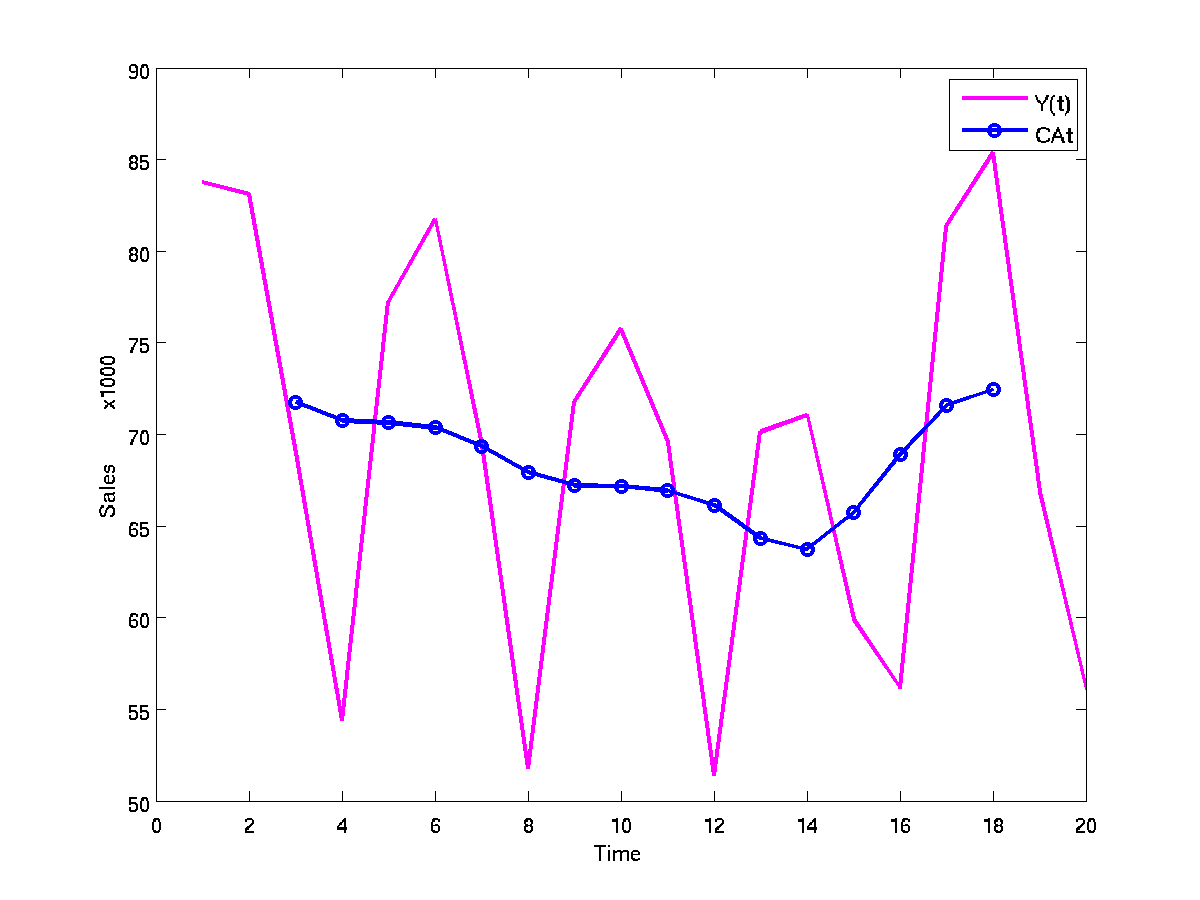
\includegraphics[totalheight=3.2in,angle=0]{graff2.png}
  \caption{Εξομάλυνση των δεδομένων του παραδείγματος 3.1 με κεντρικό κινητό μέσο.}
%  \label{fig:figure5}
\end{figure}
 
\begin{figure} [ht]
  \centering
  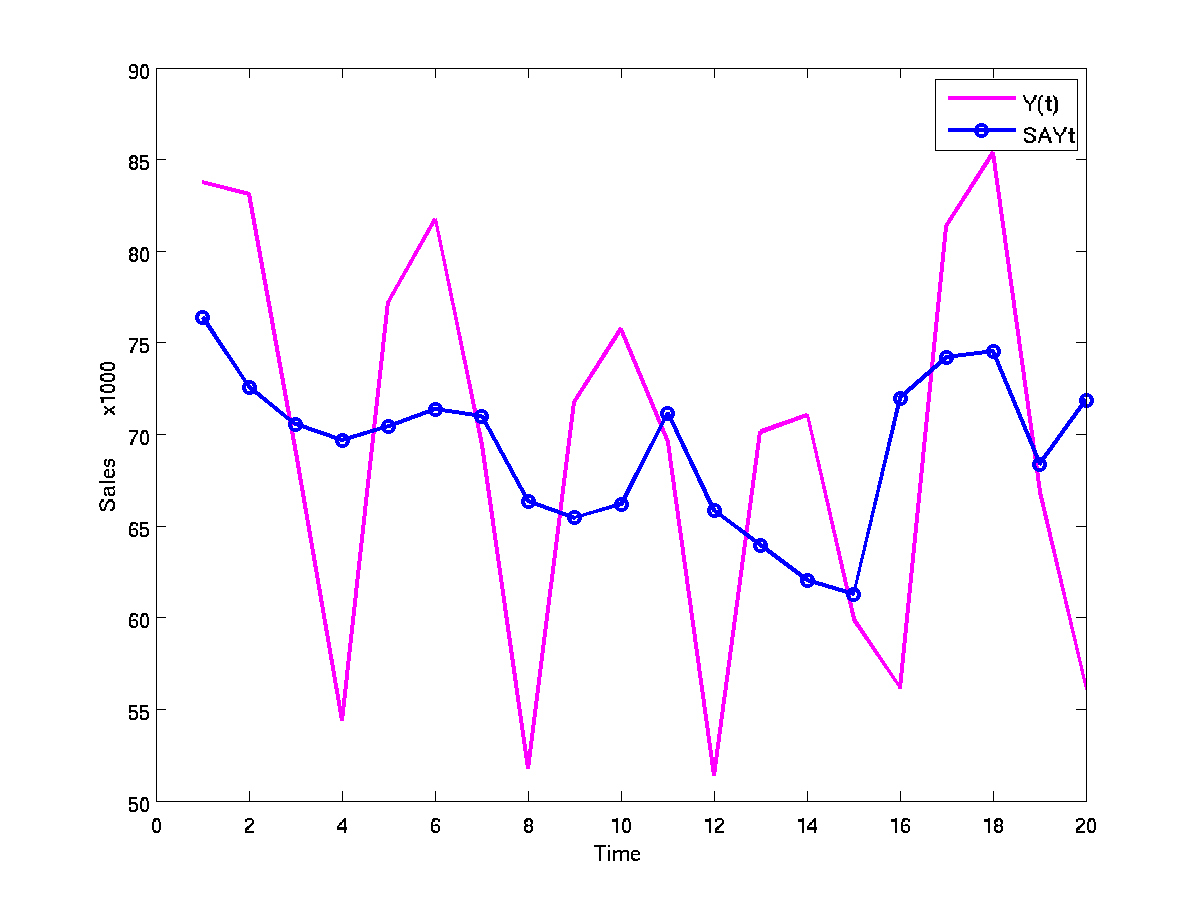
\includegraphics[totalheight=3.2in,angle=0]{graff3.png}
  \caption{Πραγματικές και απαλλαγμένες από εποχικότητα τιμές της χρονοσειράς του παραδείγματος 3.1.}
\end{figure}

\begin{table} [h]
  \caption{Προσδιορισμός Μακοχρόνιας Τάσης για τις πωλήσεις αυτοκινήτων.} 
  \label{tab_3}
  \begin{center}
    \begin{tabular}{|c|c|c|c|c|c|c|c|}
      \hline
           &   &    &    &         
           &   &    &      \\
           &    &     &    & Τιμές
           &  &     &  \\
           &  &  &  &Απαλλαγμένες &  &  &\\
       Έτος &Τρίμηνο  &Περίοδος  &Πωλήσεις  &Εποχικότητας  &  &  & Τάση \\
       & & t  & $Y_t$  & $ SAY_t$  & $t^2$  & $t*SAY_t$  &   \\
      \hline \hline
      2000 &  1o  &  1  &  83.754  &  76.371,48  &  1  & 76.371,48  &  70.551,67\\
           &  2o  &  2  &  83.121  &  72.576,98  &  4  & 145.153,96  &  70.415,93\\
           & 3ο & 3  &  68.976 & 70.538,78  & 9  & 211.616,34 & 70.280,20 \\
           & 4ο & 4 & 54.371 & 69.687,79 & 16  & 278.751,16 & 70.144,46 \\
           
        2001   & 1ο & 5  & 77.253  & 70.443,51  &  25 & 352.217,55 &  70.008,73\\
        & 2ο & 6 & 81.755 & 71.384,26 & 36  & 428.305,56 & 69.873,00\\
        & 3ο & 7  &69.424  & 70.996,93 & 49 & 496.978,51 & 69.737,26\\
        & 4ο &8  & 51.782 & 66.369,44 & 64 & 530.955,52 & 69.601,53\\
     2002   & 1o & 9 & 71.772 & 65.445,64 & 81 & 589.010,76 & 69.465,80 \\
     & 2o  & 10 & 75.771 & 66.159,34 & 100 & 661.593,40 & 69.330,06\\
     & 3o & 11 & 69.573 & 71.149,30 & 121 & 782.642,30 & 69.194,33\\
     & 4o & 12 & 51.373 & 65.845,22 &  144 & 790.142,64 &69.058,60\\
   2003  & 1o & 13 &70.153  & 63.969,34 & 169 & 831.601,42  &68.922,86\\
     & 2o & 14 &71.067 & 62.052,05 & 196 & 868.728,70 & 68.787,13\\
     & 3o & 15 & 59.909  & 61.266,35 & 225  & 918.995,25 &68.651,40\\
      & 4o & 16 & 56.164 & 71.985,89 & 256 & 1.151.774,24 & 68.515,66\\
      2004& 1o &  17& 81.377 & 74.204,00 & 289 & 1.261.468,00 & 68.379,93\\
      & 2o & 18 & 85.368 & 74.538,95  & 324 & 1.341.701,10 &68.244,20\\
      & 3o &19  & 66.868 & 68.383,02 & 361 & 1.299.277,38 &68.108,46\\
      & 4o & 20 & 56.078 & 71.875,66 & 400 & 1.437.513,20 &67.972,73\\    
      \hline
    \end{tabular}
  \end{center}
\end{table}
%%%%%%%%%%% mou ta emfanizei pio panw auta ta logia
Παρακάτω δίνεται η γραφική παράσταση των απαλλαγμένων από εποχικότητα τιμών της χρονοσειράς καθώς επίσης και η γραφική παράσταση της εκτιμηθείσας γραμμικής τάσης των τιμών της
χρονοσειράς.

\begin{figure} [ht]
  \centering
  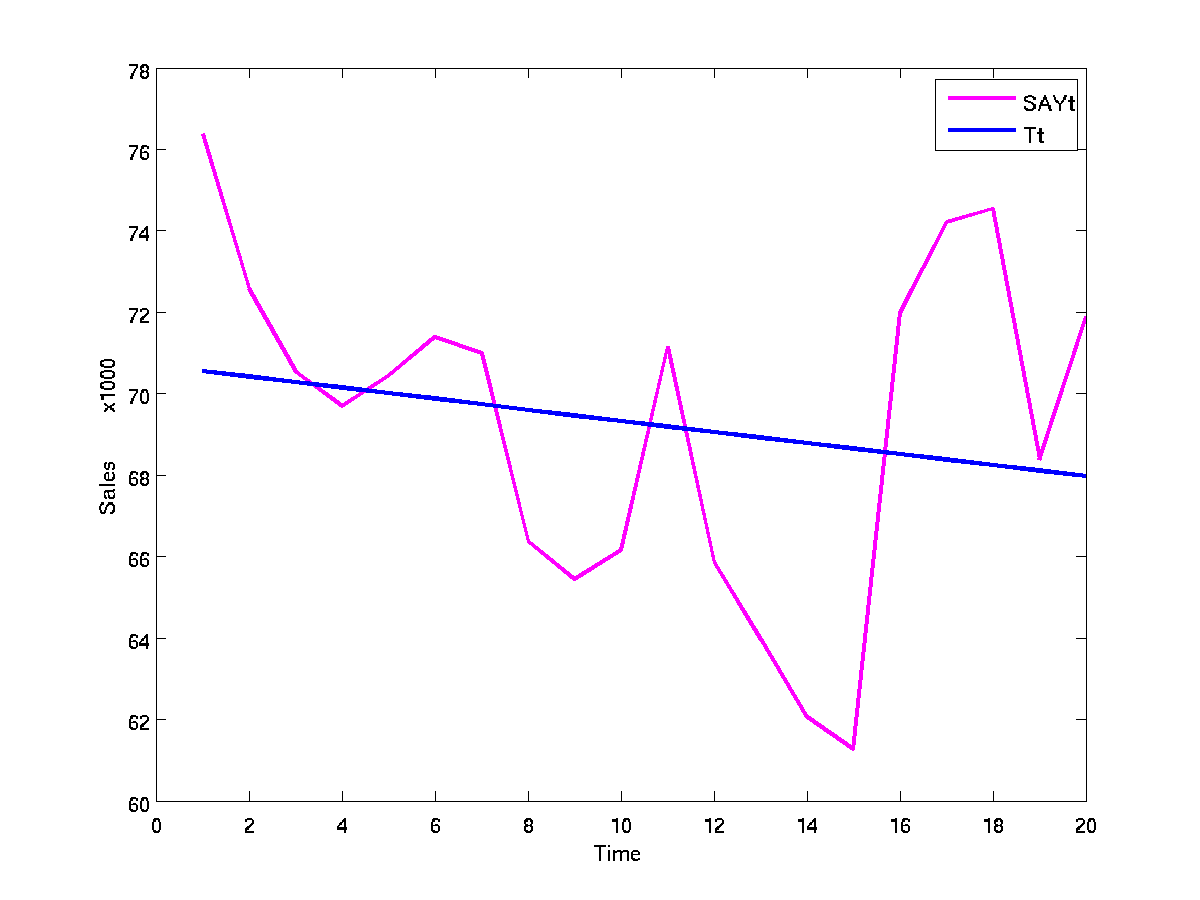
\includegraphics[totalheight=4in,angle=0]{graff4.png}
  \caption{Τιμές χρονοσειράς απαλλαγμένες από εποχικότητα και οι αντίστοιχες τιμές της τάσης του παραδείγματος 3.1.}
\end{figure}


\begin{table} [h]
  \caption{Προσδιορισμός Κυκλικών Διακυμάνσεων των πωλήσεων των αυτοκινήτων.} 
  \label{tab_4}
  \begin{center}
    \begin{tabular}{|c|c|c|c|c|c|c|c|}
      \hline
           &   &   &   &
           &   &  &Σταθμισμ.      \\
           &   &   &
           & Τιμές   &     &Τιμές    & κεντρικός   \\
          &   &   & 
           &Απαλλαγμένες  &  &Απαλλαγμένες  &κιν. Μέσος  \\
          Έτος  &Τρίμηνο  & Περίοδος & Πωλήσεις
            &Εποχικότητας  & Τάση  & από Τάση   &Όρος  \\
        &  & t  &$ Y_t$  &$ SAY_t$  &  & $ TAY_t$ & $ WA_t$ \\
      \hline \hline
      2000 &  1o  &  1  &  83.754  &  76.371,48  &  70.551,67  & 1,082  &  -\\
           &  2o  &  2  &  83.121  &  72.576,98  &  70.415,93  & 1,031  &  1,037\\
           & 3ο & 3  &  68.976 & 70.538,78  & 70.280,20  & 1,004 & 1,008 \\
           & 4ο & 4 & 54.371 & 69.687,79 & 70.144,46  & 0,993 & 0,999 \\
           
        2001   & 1ο & 5  & 77.253  & 70.443,51  &  70.008,73 & 1,006 &  1,007\\
        & 2ο & 6 & 81.755 & 71.384,26 & 69.873,00  & 1,022 & 1,017\\
        & 3ο & 7  &69.424  & 70.996,93 & 69.737,26 & 1,018 &1,003 \\
        & 4ο &8  & 51.782 & 66.369,44 & 69.601,53 & 0,954 & 0,967\\
     2002   & 1o & 9 & 71.772 & 65.445,64 & 69.465,80 & 0,942 & 0,948 \\
     & 2o  & 10 & 75.771 & 66.159,34 & 69.330,06 & 0,954 & 0,970\\
     & 3o & 11 & 69.573 & 71.149,30 & 69.194,33 & 1,028 & 0,991\\
     & 4o & 12 & 51.373 & 65.845,22 &  69.058,60 & 0,953 &0,966\\
   2003  & 1o & 13 &70.153  & 63.969,34 & 68.922,86 & 0,928  &0,928\\
     & 2o & 14 &71.067 & 62.052,05 & 68.787,13 & 0,902& 0,906\\
     & 3o & 15 & 59.909  & 61.266,35 &68.651,40  & 0,892 &0,934\\
      & 4o & 16 & 56.164 & 71.985,89 & 68.515,66 & 1,051 & 1,020\\
      2004& 1o &  17& 81.377 & 74.204,00 & 68.379,93 & 1,085 & 1,078\\
      & 2o & 18 & 85.368 & 74.538,95  & 68.244,20 &1,092 &1,068\\
      & 3o &19  & 66.868 & 68.383,02 & 68.108,46 & 1,004 &1,039\\
      & 4o & 20 & 56.078 & 71.875,66 & 67.972,73 & 1,057 &-\\
     
      \hline
    \end{tabular}
  \end{center}
\end{table}
%%%%%%%%%%%%%%mou ta emfanizei pio panw ayta ta logia
Οι απαλλαγμένες από τάση και εποχικότητα τιμές του παραπάνω παραδείγματος, περιέχουν μόνο την
κυκλικότητα και τη μη κανονικότητα. Παρακάτω δίνεται η γραφική παράσταση των απαλλαγμένων από τάση και εποχικότητα τιμών της χρονοσειράς (TAYt) και η γραφική παράσταση των τιμών του σταθμικού κεντρικού κινητού μέσου (WAt).
\begin{figure} [ht]
  \centering
  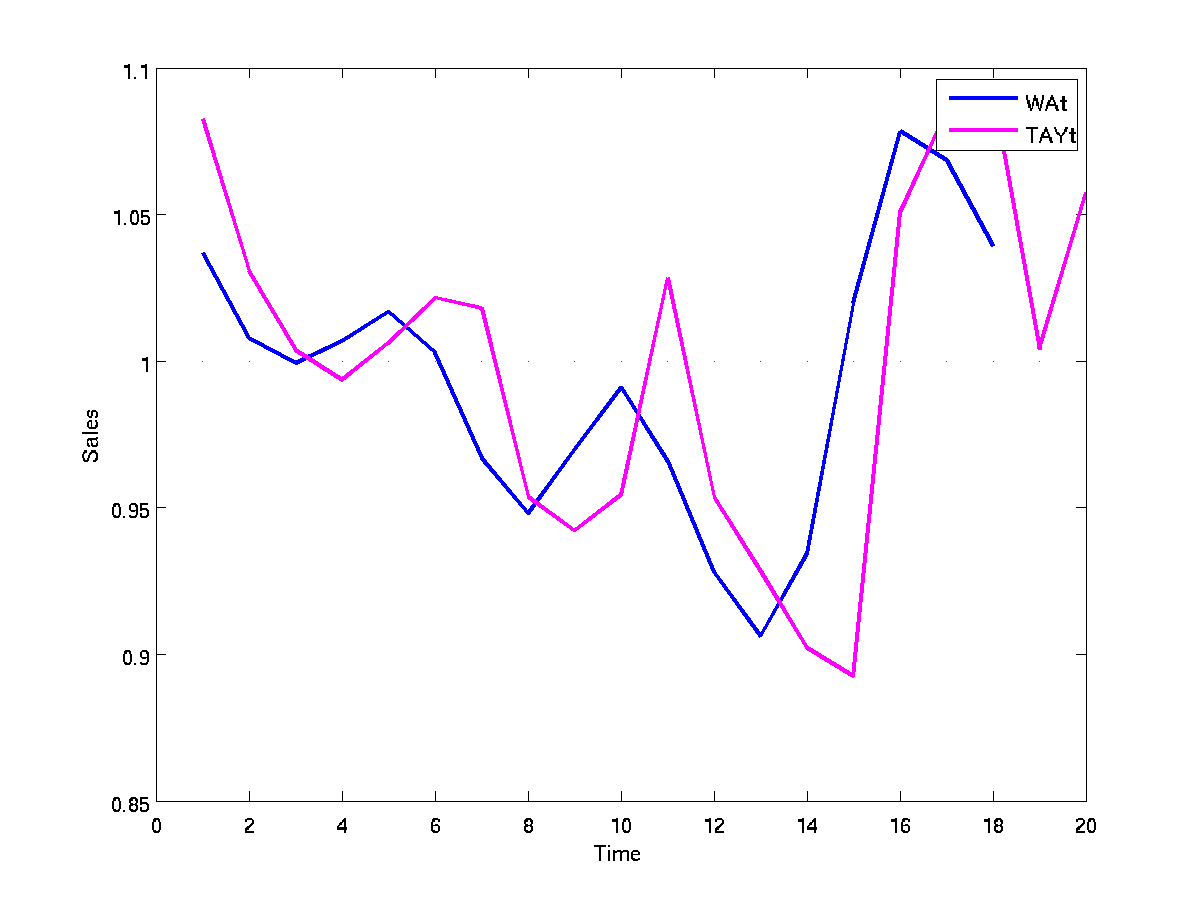
\includegraphics[totalheight=3.2in,angle=0]{graff6.png}
  \caption{Τιμές χρονοσειράς απαλλαγμένες από τάση και από εποχικότητα του παραδείγματος 3.1 και τιμές του σταθμικού κεντρικού κινητού μέσου.}
\end{figure}

\begin{table} [h]
  \caption{Προβλέψεις για τα επόμενα δύο έτη.} 
  \label{tab_5}
  \begin{center}
    \begin{tabular}{|c |c | c| c|}
      \hline 
       &  &  &  \\
       Έτος &Τρίμηνο   &Περίοδος   &Προβλέψεις  \\
       &   & t  & $\widehat{Y}_t$  \\    
       \hline \hline
       2005 & 1o & 21 & 74.395 \\
            & 2o & 22 & 77.537 \\
            & 3o & 23 & 66.069 \\
            & 4o & 24 & 52.609 \\
       2006 & 1o & 25 & 73.799 \\
            & 2o & 26 & 76.915 \\
            & 3o & 27 & 65.538 \\
            & 4o & 28 & 52.186 \\     
      \hline
    \end{tabular}
  \end{center}
\end{table}

\begin{figure} [ht]
  \centering
  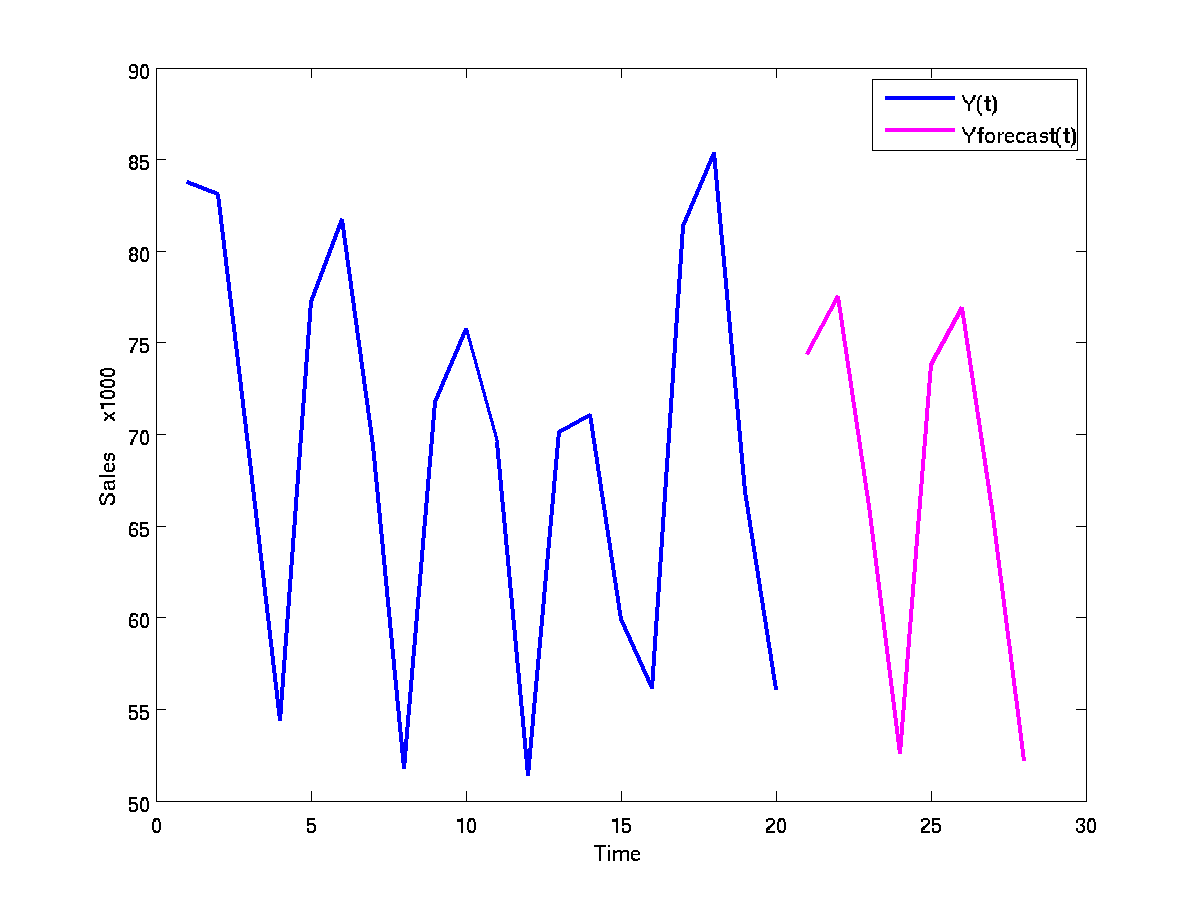
\includegraphics[totalheight=3.2in,angle=0]{graff7.png}
  \caption{Πραγματικές τιμές της χρονοσειράς και οι προβλεπόμενες τιμές για το έκτο και έβδομο έτος.}
\end{figure}

\begin{table} [h]
  \caption{Προσδιορισμός Κυκλικών Διακυμάνσεων των πωλήσεων των αυτοκινήτων.} 
  \label{tab_4}
  \begin{center}
    \begin{tabular}{|c|c|c|c|c|c|c|c|c|}
      \hline
           &   &   &   &
           &   &  &   &     \\
           Έτος & Τρίμηνο  & Πείοδος  & Πωλήσεις  & $ A_t$
           & $T_t$   & $ S_t$  & $ \widehat{Y}_t$  & $ e_t$ \\
      \hline \hline
      2000 &  1o  &  1  &  83.754  &    &     & 1,15 &  & \\
           &  2o  &  2  &  83.121  &    &   & 1,15  &  & \\
           & 3ο & 3  &  68.976 &   &  & 0,95 &  &  \\
           & 4ο & 4 & 54.371 & 72.555,50 & 0,00  & 0,75 &  &  \\
           
        2001   & 1ο & 5  & 77.253  & 69.121,08  & -34,34 & 1,14 & 83.754,00 & -6.501,00\\
        & 2ο & 6 & 81.755 & 70.474,95 & -20,46  & 1,15 & 79.147,11 &2.607,89 \\
        & 3ο & 7  &69.424  & 72.023,13 & -4,78 & 0,95 &66.978,64 & 2.445,36 \\
        & 4ο &8  & 51.782 & 70.239,02 & -22,57 & 0,75 & 53.968,48 & -2.186,48\\
     2002   & 1o & 9 & 71.772 & 65.700,57 & -67,73 & 1,13 & 80.233,57 & -8.461,57 \\
     & 2o  & 10 & 75.771 & 65.780,78 & -66,25 & 1,15 & 75.491,97 & 279,03\\
     & 3o & 11 & 69.573 & 70.072,20 & -22,67 & 0,97 & 62.749,69 & 6.823,31\\
     & 4o & 12 & 51.373 & 69.354,86 & -29,62 & 0,74 &52.222,22 & -849,22\\
   2003  & 1o & 13 &70.153  & 65.020,45 & -72,67 & 1,11  &78.106,10 &-7.953,10\\
     & 2o & 14 &71.067 & 63.002,24 & -92,12 & 1,14& 74.738,23 & -3.671,23\\
     & 3o & 15 & 59.909  & 62.327,53 & -97,95  & 0,97 & 60.832,78 & -923,78\\
      & 4o & 16 & 56.164 & 70.316,76 & -17,08 & 0,76 & 46.297,77 & 9.866,23\\
      2004& 1o &  17& 81.377 & 72.078,03 & 0,71 & 1,12 & 78.135,81 &3.241,19 \\
      & 2o & 18 & 85.368 & 73.649,64  & 16,42 & 1,15 & 82.422,38 &2.945,62 \\
      & 3o &19  & 66.868 & 70.993,35 & -10,31 & 0,96 &71.097,92 &-4.229,92 \\
      & 4o & 20 & 56.078 & 72.609,38 & 5,95 & 0,76 &54.047,41 & 2.030,59\\
      2005 & 1o  & 21 &  &  &  &  &81.115  &  \\
      & 2o & 22 &  &  &  &  & 83.404  &  \\
      & 3o & 23 &  &  &  &  & 69.558 &  \\
      & 4o & 24 &  &  &  &  & 55.556  &  \\
      2006& 1o & 25 &  &  &  &  & 81.142 &  \\
      & 2o &26  &  &  &  &  & 83.431 &  \\
      & 3o & 27 &  &  &  &  &69.581  &  \\
      & 4o & 28 &  &  &  &  & 55.574 &  \\
     
      \hline
    \end{tabular}
  \end{center}
\end{table}
%\begin{center}
%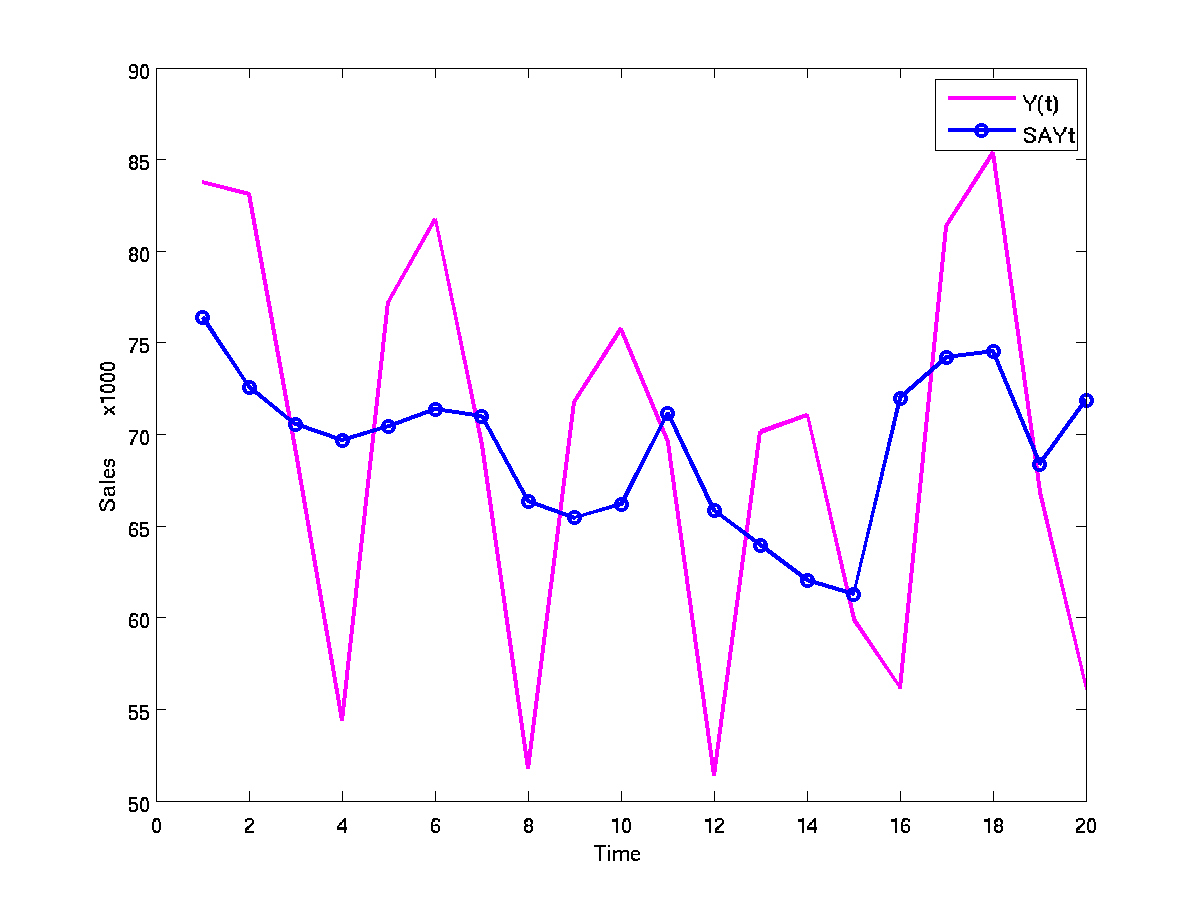
\includegraphics[scale=0.7]{graff3.png}\\   
%\textbf{Σχήμα 3.1: Γράφημα χρονοσειράς}
%\end{center} 
%%%%%%%%%%%%%%%%%%%%%%%%%%%%%%%%%%%%%%%%%%%%%%%%%%%%%%%%%%%%%%%%%%%%%%%%%%%%%%%%%%%%%%%%%%%%%%%%%%%%
%\subsection{Όνομα πρώτης υποενότητας}
%%%%%%%%%%%%%%%%%%%%%%%%%%%%%%%%%%%%%%%%%%%%%%%%%%%%%%%%%%%%%%%%%%%%%%%%%%%%%%%%%%%%%%%%%%%%%%%%%%%%
%%%%%%%%%%%%%%%%%%%%%%%%%%%%%%%%%%%%%%%%%%%%%%%%%%%%%%%%%%%
%\section{ΒΡΑΧΥΠΡΟΘΕΣΜΕΣ ΠΡΟΒΛΕΨΕΙΣ ΧΡΗΣΙΜΟΠΟΙΩΝΤΑΣ ΤΗ ΜΕΘΟΔΟ WINTERS}
%%%%%%%%%%%%%%%%%%%%%%%%%%%%%%%%%%%%%%%%%%%%%%%%%%%%%%%%%%%





%%%%%%%%%%%%%%% File ends here %%%%%%%%%%%%%%%%%%%%%%%%%%%%%%%%
\endinput
%%% Local Variables: 
%%% mode: latex
%%% TeX-master: "ptyxiakn"
%%% End: 


\include{chapter4}

%%%%%%%%%%%%%%%% Apendices  %%%%%%%%%%%%%%%%%%
\appendix
%%%%%%%%%%%%%%%%%%%%%%%%%%%%%%%%%%%%%%%%%%%%%%%%%%%%%%%%%%%%%%%%%%%%%
\chapter[Concentration for uniformely\ldots]{The concentration property 
for uniformly convex bodies contained in small Euclidean balls}
%%%%%%%%%%%%%%%%%%%%%%%%%%%%%%%%%%%%%%%%%%%%%%%%%%%%%%%%%%%%%%%%%%%%%

\endinput
%%% Local Variables: 
%%% mode: latex
%%% TeX-master: "ptyxiakn"
%%% End: 

\include{appendix2}
\include{appendix3}
%%%%%%%%%%%%%%%%%%%%%%%%%%%%%%%%%%%%%%%%%%%%%%

%%%%%%%%%%% Back matter starts %%%%%%%%%%%%%%%
\backmatter
%%%%%%%%%%%%%%%%%%%%%%%%%%%%%%%%%%%%%%%%%%%%%%

\printindex

\clearpage

\addcontentsline{toc}{chapter}{Βιβλιογραφία}
\bibliographystyle{plain}      % mathematics and physical sciences
\bibliography{ptyxiakh}

\end{document}
%%% Local Variables: 
%%% mode: latex
%%% TeX-master: t
%%% End: 
